\documentclass[a4paper,14pt]{extarticle}
\usepackage[utf8]{inputenc}
\usepackage[russian]{babel}
\usepackage{graphicx}
\usepackage[top=1in, bottom=1in, left=1in, right=1in]{geometry}
\usepackage{pgfplots}
\usepackage{amsmath}
\usepackage{setspace}
\usepackage{titlesec}
\usepackage{float}
\usepackage{chngcntr}
\usepackage{pgfplots}
\usepackage{amsfonts}
\usepackage{pgfplotstable}
\usepackage{multirow}
\usepackage{karnaugh-map}
\usepackage{tikz,xcolor}
\usepackage{tkz-graph}
\usepackage{tabularx}
    \newcolumntype{L}{>{\centering\arraybackslash}X}
\renewcommand{\arraystretch}{1.2}
\usetikzlibrary{arrows, petri, topaths}

\titleformat{\section}[hang]
  {\bfseries}
  {}
  {0em}
  {\hspace{-0.4pt}\large \thesection\hspace{0.6em}}
  
  
\titleformat{\subsection}[hang]
  {\bfseries}
  {}
  {0em}
  {\hspace{-0.4pt}\large \thesubsection\hspace{0.6em}}

%\linespread{1.3} % полуторный интервал
%\renewcommand{\rmdefault}{ftm} % Times New Roman

\newcommand{\nx}{\overline{x}}
\newcommand{\p}{0.31}
\newcommand{\scale}{1.4}

\counterwithin{figure}{section}
\counterwithin{equation}{section}
\counterwithin{table}{section}

\begin{document}
\begin{titlepage}
\centering
Санкт-Петербургский политехнический университет Петра Великого \\
\vspace{0.15cm}
Кафедра компьютерных систем и программных технологий \\
\vspace{6.5cm}

{\centering \textbf{Отчёт по расчетному заданию} \\ 
\vspace{0.15cm}
\textbf{Дисциплина}: Системный анализ \\
\vspace{0.15cm}
\textbf{Тема}: Теория расписаний} \\

\vspace{6.5cm}

\begin{table}[H]
\begin{tabular}{p{\textwidth}@{}r}
{Выполнил студент гр. 33501/4} \hfill {Леженин Ю.И.} \\
{Преподаватель} \hfill {Сабонис С.С.} \\
\end{tabular}
\end{table}
\vfill

{\centering Санкт-Петербург \\ 
\vspace{0.15cm}
\today}
\end{titlepage}

\section{Исходные данные}

\begin{center}
\large{Вариант 40}
\end{center}

\begin{figure}[h]
\centering
\begin{tikzpicture}
\SetGraphUnit{4}  

\Vertex[x=3, y=3]{1}
\Vertex[x=3, y=0]{2}
\Vertex[x=6, y=3]{3}
\Vertex[x=6, y=-1.5]{5}
\Vertex[x=9, y=0]{7}

\Vertex[x=0, y=0]{0}
\Vertex[x=3, y=-3]{4}
\Vertex[x=9, y=-3]{6}
\Vertex[x=12, y=0]{8}

\tikzstyle{EdgeStyle}=[post]

\Edge[label = {3}](0)(1)
\Edge[label = {5}](0)(2)
\Edge[label = {3}](0)(4)
\Edge[label = {6}, style={pos=.75}](0)(5)
\Edge[label = {5}](1)(3)
\Edge[label = {4}, style={pos=.75}](1)(5)
\Edge[label = {6}, style={pos=.75}](2)(3)
\Edge[label = {6}](2)(4)
\Edge[label = {7}](3)(7)
\Edge[label = {6}](4)(5)
\Edge[label = {3}](4)(6)
\Edge[label = {3}](5)(6)
\Edge[label = {3}](5)(7)
\Edge[label = {7}](6)(7)
\Edge[label = {3}](6)(8)
\Edge[label = {6}](7)(8)

\end{tikzpicture}
\caption{Исходный граф}
\label{ris:image}
\end{figure}

\section{Решение. Часть 1}

Для заданного графа была построена таблица смежности вершин и рассчитаны наиболее ранние и поздние моменты наступления событий и резервы времени выполнения работы, определен критический путь и его длина. Результаты приведены в таблицах \ref{tabular:timesandtenses}, \ref{tabular:timesandtenses1} и \ref{tabular:timesandtenses2}.

\begin{table}[H]
\caption{Матрица смежности для заданного графа}
\label{tabular:timesandtenses}
\begin{center}
\begin{tabular}{|c|c|c|c|c|c|c|c|c|c|}
\hline
  & 0 & 1 & 2 & 3 & 4 & 5 & 6 & 7 & 8\\ \hline
0 & - & 3 & 5 & - & 3 & 6 & - & - & -\\ \hline
1 & - & - & - & 5 & - & 4 & - & - & -\\ \hline
2 & - & - & - & 6 & 6 & - & - & - & -\\ \hline
3 & - & - & - & - & - & - & - & 7 & -\\ \hline
4 & - & - & - & - & - & 6 & 3 & - & -\\ \hline
5 & - & - & - & - & - & - & 3 & 3 & -\\ \hline
6 & - & - & - & - & - & - & - & 7 & 3\\ \hline
7 & - & - & - & - & - & - & - & - & 6\\ \hline
8 & - & - & - & - & - & - & - & - & -\\ \hline
\end{tabular}
\end{center}
\end{table}

Наиболее ранние моменты наступления событий определяются по формуле: 
$$t^{'}_{i} = \max ( t^{'}_{j} + \tau_{ji})), ~ j \in G^{-} (i),$$
наиболее поздние -- по формуле
$$t^{''}_{j} = \min ( t^{''}_{i} - \tau_{ji})), ~ i \in G (j),$$
где $\tau_{ji}$ -- время выполнения работы для перехода между событиями $j$ и $i$, $G^{-}$ -- множество обратного соответствия, а $G$ -- прямого.


%\newpage

%Наиболее ранние моменты наступления событий:\\\\
%
%\begin{minipage}{0.4\textwidth}
%\begin{center}
% ${t_0}^{'} = 0$ \\
% ${t_1}^{'} = 3$ \\
% ${t_2}^{'} = 5$ \\
% ${t_3}^{'} = 11$ \\
% ${t_4}^{'} = 11$
%\end{center}
%\end{minipage}
%\hfill
%\begin{minipage}{0.5\textwidth}
%\begin{center}
% ${t_5}^{'} = 17$ \\
% ${t_6}^{'} = 20$ \\
% ${t_7}^{'} = 27$ \\
% ${t_8}^{'} = 33$
%\end{center}
%\end{minipage}\\\\\\
%
%Наиболее поздние моменты наступления событий:\\\\
%
%\begin{minipage}{0.4\textwidth}
%\begin{center}
% ${t_8}^{''} = 33$ \\
% ${t_7}^{''} = 27$ \\
% ${t_6}^{''} = 20$ \\
% ${t_5}^{''} = 17$ \\
% ${t_4}^{''} = 11$
%\end{center}
%\end{minipage}
%\hfill
%\begin{minipage}{0.5\textwidth}
%\begin{center}
% ${t_3}^{''} = 20$ \\
% ${t_2}^{''} = 5$ \\
% ${t_1}^{''} = 13$ \\
% ${t_0}^{''} = 0$
%\end{center}
%\end{minipage}\\\\

\begin{table}[H]
\caption{Наиболее ранние/поздние моменты наступления событий}
\label{tabular:timesandtenses1}
\begin{center}
\begin{tabular}{|c|c|c|c|c|c|c|c|c|c|}
\hline
$i$ & 0 & 1 & 2 & 3 & 4 & 5 & 6 & 7 & 8\\ \hline
${t}^{'}_{i}$ & 0 & 3 & 5 & 11 & 11 & 17 & 20 & 27 & 33\\ \hline
${t}^{''}_{i}$ & 0 & 13 & 5 & 20 & 11 & 17 & 20 & 27 & 33\\ \hline
\end{tabular}
\end{center}
\end{table}

Резерв времени выполнения работы определяется по формуле
$$r_{ij} = t^{''}_{j} - (t^{'}_{i} + \tau_{ij}).$$

\begin{table}[H]
\caption{Таблица резервов времени}
\label{tabular:timesandtenses2}
\begin{center}
\begin{tabular}{|c|c|c|c|c|c|c|c|c|c|}
\hline
  & 0 & 1 & 2 & 3 & 4 & 5 & 6 & 7 & 8\\ \hline
0 & - & 10 & 0 & - & 8 & 11 & - & - & -\\ \hline
1 & - & - & - & 12 & - & 10 & - & - & -\\ \hline
2 & - & - & - & 9 & 0 & - & - & - & -\\ \hline
3 & - & - & - & - & - & - & - & 9 & -\\ \hline
4 & - & - & - & - & - & 0 & 6 & - & -\\ \hline
5 & - & - & - & - & - & - & 0 & 7 & -\\ \hline
6 & - & - & - & - & - & - & - & 0 & 10\\ \hline
7 & - & - & - & - & - & - & - & - & 0\\ \hline
8 & - & - & - & - & - & - & - & - & -\\ \hline
\end{tabular}
\end{center}
\end{table}

Критический путь: \ 0 $\rightarrow$ 2 $\rightarrow$ 4 $\rightarrow$ 5 $\rightarrow$ 6 $\rightarrow$ 7 $\rightarrow$ 8.

Длина пути: \ 33

\section{Решение. Часть 2}

Для числа рабочих $N = 1$ общее время выполнения будет равно сумме времени выполнения всех работ, т.е. $T = 76$ \\\\
Для числа рабочих $N = 3$ в таблицах \ref{tabular:timesandtenses3} - \ref{tabular:timesandtenses6} приведены оценки времени полученные с помощью четырех различных методов. \\\\
Используемые обозначения: \\
T -- затраченное время \\
D -- законченные работы \\
E -- произошедшие события \\
W -- доступные работы \\
A -- длительность выполнения  \\
B -- выбранные для исполнения работы \\
L -- время, через которое окончится выполнение работы


\newpage
\subsection{Максимальная длительность работы.}


\begin{table}[H]
\caption{Пошаговое выполнение. Критерий выбора работ: максимальная длительность.}
\label{tabular:timesandtenses3}
\small
\begin{center}
\begin{tabularx}{\linewidth}{|L|L|L|L|L|L|L|}
\hline
T & D & E & W & A & B & L\\ \hline
0 & [~] & [0] & [0 1] [0 2] [0 4] [0 5] & [3 5 3 6] & [0 5] [0 2] [0 1] & [6 5 3] \\ \hline 
 3 & [0 1] & [0 1] & [0 4] [1 3] [1 5] & [3 5 4] & [0 5] [0 2] [1  3] & [3 2 5] \\ \hline 
 5 & [0 2] & [0 1 2] & [0  4]  [1  5]  [2  3]  [2  4] & [3  4  6  6] & [0  5]  [1  3]  [2  3] & [1  3  6] \\ \hline 
 6 & [0 5] & [0 1 2] & [0  4]  [1  5]  [2  4] & [3  4  6] & [1  3]  [2  3]  [2  4] & [2  5  6] \\ \hline 
 8 & [1 3] & [0 1 2] & [0  4]  [1  5] & [3  4] & [2  3]  [2  4]  [1  5] & [3  4  4] \\ \hline 
 11 & [2 3] & [0 1 2 3] & [0  4]  [3  7] & [3  7] & [2  4]  [1  5]  [3  7] & [1  1  7] \\ \hline 
 12 & [2 4]
 [1 5] & [0 1 2 3] & [0  4] & [3] & [3  7]  [0  4] & [6  3] \\ \hline 
 15 & [0 4] & [0 1 2 3 4] & [4  5]  [4  6] & [6  3] & [3  7]  [4  5]  [4  6] & [3  6  3] \\ \hline 
 18 & [3 7]
 [4 6] & [0 1 2 3 4] & [~] & [~] & [4  5] & [3] \\ \hline 
 21 & [4 5] & [0 1 2 3 4 5] & [5  6]  [5  7] & [3  3] & [5  6]  [5  7] & [3  3] \\ \hline 
 24 & [5 6]
 [5 7] & [0 1 2 3 4 5 6] & [6  7]  [6  8] & [7  3] & [6  7]  [6  8] & [7  3] \\ \hline 
 27 & [6 8] & [0 1 2 3 4 5 6] & [~] & [~] & [6  7] & [4] \\ \hline 
 31 & [6 7] & [0 1 2 3 4 5 6 7] & [7  8] & [6] & [7  8] & [6] \\ \hline 
 37 & [7 8] & [0 1 2 3 4 5 6 7 8] & [~] & [~] & [~] & [~] \\ \hline 
\end{tabularx}
\end{center}
\end{table}
\noindent

Общее время: 37 \\
1-й исполнитель простаивал 0 часов\\
2-й исполнитель простаивал 13 часов \\
3-й исполнитель простаивал 22 часа \\

\begin{figure}[H]
\centering
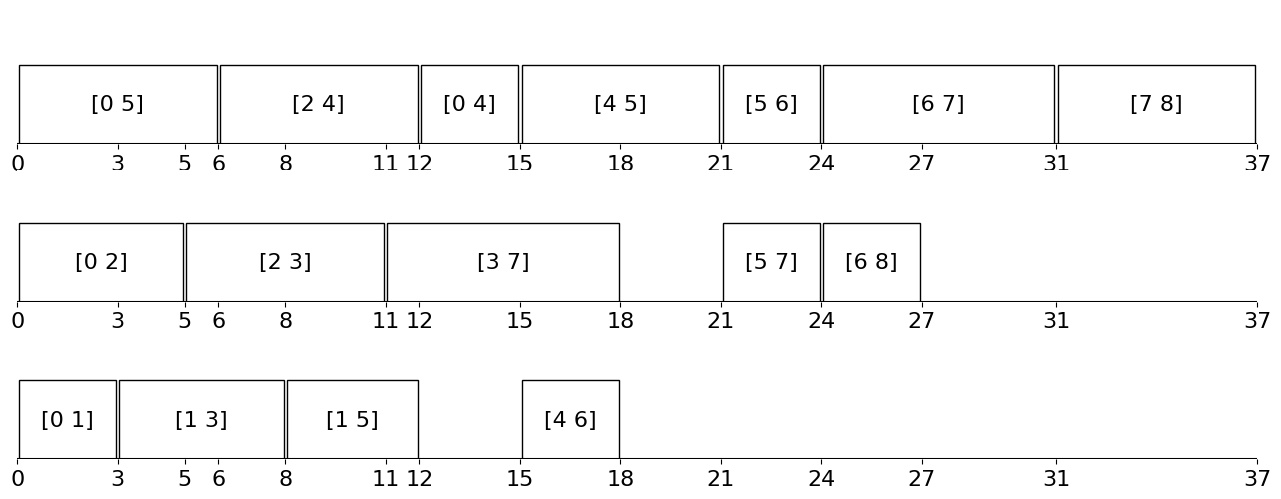
\includegraphics[width=1\linewidth]{diag1.png}
\caption{Диаграмма распределения. Критерий выбора работ максимальная длительность.}
\label{ris:image1}
\end{figure}


\subsection{Минимальная длительность работы.}


\begin{table}[H]
\caption{Пошаговое выполнение. Критерий выбора работ: минимальная длительность.}
\label{tabular:timesandtenses4}
\small
\begin{center}
\begin{tabularx}{\linewidth}{|L|L|L|L|L|L|L|}
\hline
T & D & E & W & A & B & L\\ \hline
0 & [~] & [0] & [0 1] [0 2] [0 4] [0 5] & [3 5 3 6] & [0 1] [0 4] [0 2] & [3 3 5] \\ \hline 
3 & [0 1] [0 4] & [0 1] & [0 5] [1 3] [1 5] & [6 5 4] & [0 2] [1 5] [1 3] & [2 4 5] \\ \hline 
5 & [0 2] & [0 1 2] & [0 5] [2 3] [2 4] & [6 6 6] & [1 5] [1 3] [0 5] & [2 3 6] \\ \hline 
7 & [1 5] & [0 1 2] & [2 3] [2 4] & [6 6] & [1 3] [0 5] [2 3] & [1 4 6] \\ \hline 
8 & [1 3] & [0 1 2] & [2 4] & [6] & [0 5] [2 3] [2 4] & [3 5 6] \\ \hline 
11 & [0 5] & [0 1 2] & [~] & [~] & [2 3] [2 4] & [2 3] \\ \hline 
13 & [2 3] & [0 1 2 3] & [3 7] & [7] & [2 4] [3 7] & [1 7] \\ \hline 
14 & [2 4] & [0 1 2 3 4] & [4 5] [4 6] & [6 3] & [3 7] [4 6] [4 5] & [6 3 6] \\ \hline 
17 & [4 6] & [0 1 2 3 4] & [~] & [~] & [3 7] [4 5] & [3 3] \\ \hline 
20 & [3 7] [4 5] & [0 1 2 3 4 5] & [5 6] [5 7] & [3 3] & [5 6] [5 7] & [3 3] \\ \hline 
23 & [5 6] [5 7] & [0 1 2 3 4 5 6] & [6 7] [6 8] & [7 3] & [6 8] [6 7] & [3 7] \\ \hline 
26 & [6 8] & [0 1 2 3 4 5 6] & [~] & [~] & [6 7] & [4] \\ \hline 
30 & [6 7] & [0 1 2 3 4 5 6 7] & [7 8] & [6] & [7 8] & [6] \\ \hline 
36 & [7 8] & [0 1 2 3 4 5 6 7 8] & [~] & [~] & [~] & [~] \\ \hline 
\end{tabularx}
\end{center}
\end{table}

Общее время: 37 \\
1-й исполнитель простаивал 4 часа\\
2-й исполнитель простаивал 9 часов \\
3-й исполнитель простаивал 19 часов \\

\begin{figure}[H]
\center{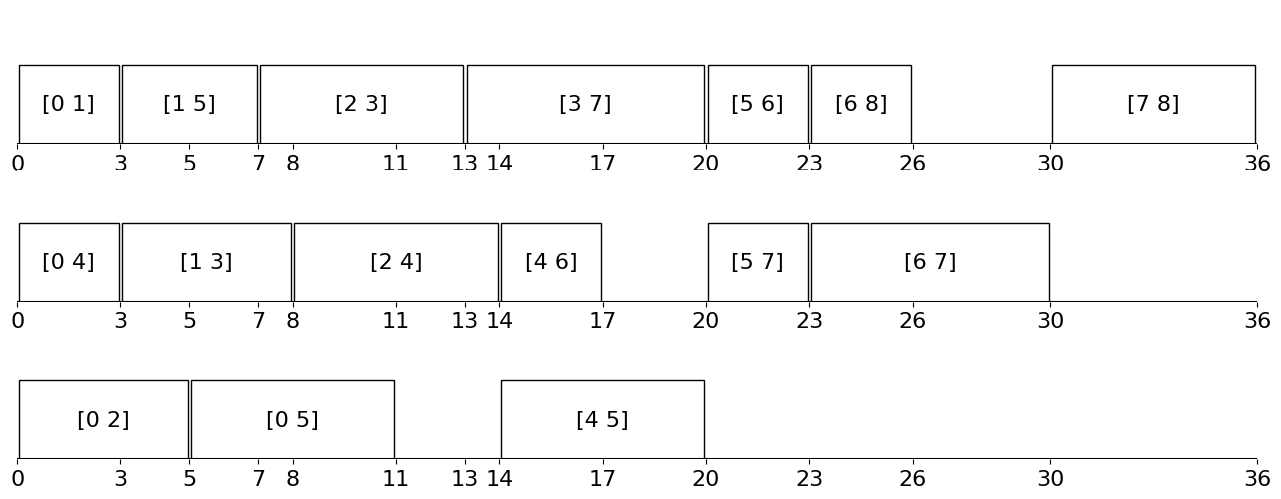
\includegraphics[width=1\linewidth]{diag2.png}}
\caption{Диаграмма распределения. Критерий выбора работ: минимальная длительность.}
\label{ris:image}
\end{figure}

\newpage
\subsection{Наименьший резерв.}

\begin{table}[H]
\caption{Пошаговое выполнение. Критерий выбора работы: наименьший резерв.}
\label{tabular:timesandtenses5}
\small
\begin{center}
\begin{tabularx}{\linewidth}{|L|L|L|L|L|L|L|}
\hline
T & D & E & W & A & B & L\\ \hline
0 & [~] & [0] & [0 1] [0 2] [0 4] [0 5] & [3 5 3 6] & [0 5] [0 1] [0 4] & [6 3 3] \\ \hline 
3 & [0 1] [0 4] & [0 1] & [0 2] [1 3] [1 5] & [5 5 4] & [0 5] [1 3] [1 5] & [3 5 4] \\ \hline 
6 & [0 5] & [0 1] & [0 2] & [5] & [1 3] [1 5] [0 2] & [2 1 5] \\ \hline 
7 & [1 5] & [0 1] & [~] & [~] & [1 3] [0 2] & [1 4] \\ \hline 
8 & [1 3] & [0 1] & [~] & [~] & [0 2] & [3] \\ \hline 
11 & [0 2] & [0 1 2] & [2 3] [2 4] & [6 6] & [2 3] [2 4] & [6 6] \\ \hline 
17 & [2 3] [2 4] & [0 1 2 3 4] & [3 7] [4 5] [4 6] & [7 6 3] & [3 7] [4 6] [4 5] & [7 3 6] \\ \hline 
20 & [4 6] & [0 1 2 3 4] & [~] & [~] & [3 7] [4 5] & [4 3] \\ \hline 
23 & [4 5] & [0 1 2 3 4 5] & [5 6] [5 7] & [3 3] & [3 7] [5 7] [5 6] & [1 3 3] \\ \hline 
24 & [3 7] & [0 1 2 3 4 5] & [~] & [~] & [5 7] [5 6] & [2 2] \\ \hline 
26 & [5 7] [5 6] & [0 1 2 3 4 5 6] & [6 7] [6 8] & [7 3] & [6 8] [6 7] & [3 7] \\ \hline 
29 & [6 8] & [0 1 2 3 4 5 6] & [~] & [~] & [6 7] & [4] \\ \hline 
33 & [6 7] & [0 1 2 3 4 5 6 7] & [7 8] & [6] & [7 8] & [6] \\ \hline 
39 & [7 8] & [0 1 2 3 4 5 6 7 8] & [~] & [~] & [~] & [~] \\ \hline
\end{tabularx}
\end{center}
\end{table}


\begin{figure}[H]
\center{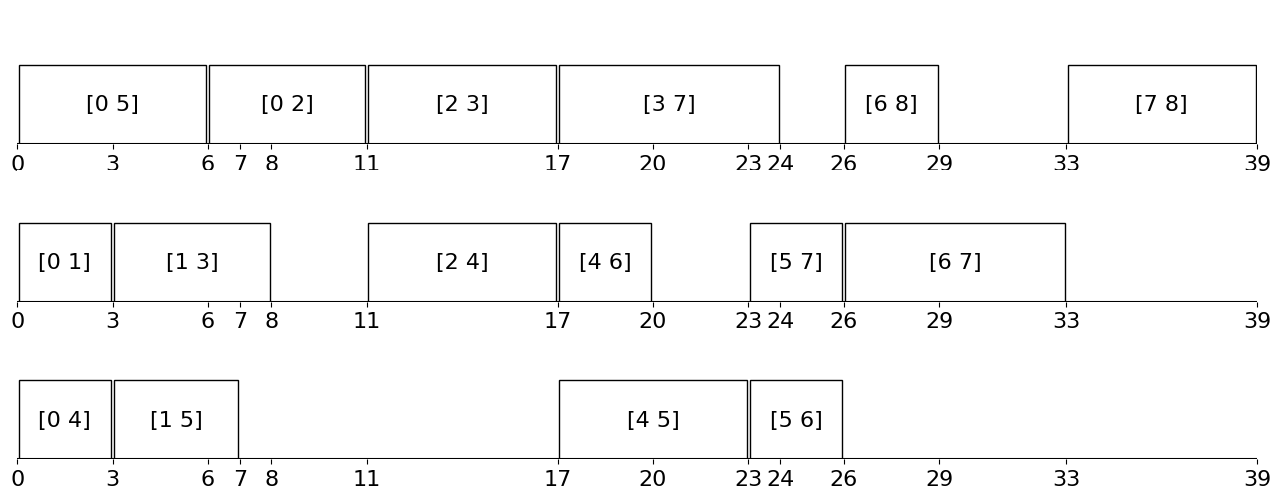
\includegraphics[width=1\linewidth]{diag3.png}}
\caption{Диаграмма распределения. Критерий выбора работ: наименьший резерв.}
\label{ris:image}
\end{figure}

Общее время: 33 \\
1-й исполнитель простаивал 0 часов\\
2-й исполнитель простаивал 11 часов \\
3-й исполнитель простаивал 22 часов \\


\subsection{Наибольший резерв.}

\begin{table}[H]
\caption{ППошаговое выполнение. Критерий выбора работы: наибольший резерв.}
\label{tabular:timesandtenses6}
\small
\begin{center}
\begin{tabularx}{\linewidth}{|L|L|L|L|L|L|L|}
\hline
T & D & E & W & A & B & L\\ \hline
0 & [~] & [0] & [0 1] [0 2] [0 4] [0 5] & [3 5 3 6] & [0 2] [0 4] [0 1] & [5 3 3] \\ \hline 
3 & [0 4] [0 1] & [0 1] & [0 5] [1 3] [1 5] & [6 5 4] & [0 2] [1 5] [0 5] & [2 4 6] \\ \hline 
5 & [0 2] & [0 1 2] & [1 3] [2 3] [2 4] & [5 6 6] & [1 5] [0 5] [2 4] & [2 4 6] \\ \hline 
7 & [1 5] & [0 1 2] & [1 3] [2 3] & [5 6] & [0 5] [2 4] [2 3] & [2 4 6] \\ \hline 
9 & [0 5] & [0 1 2] & [1 3] & [5] & [2 4] [2 3] [1 3] & [2 4 5] \\ \hline 
11 & [2 4] & [0 1 2 4] & [4 5] [4 6] & [6 3] & [2 3] [1 3] [4 5] & [2 3 6] \\ \hline 
13 & [2 3] & [0 1 2 4] & [4 6] & [3] & [1 3] [4 5] [4 6] & [1 4 3] \\ \hline 
14 & [1 3] & [0 1 2 3 4] & [3 7] & [7] & [4 5] [4 6] [3 7] & [3 2 7] \\ \hline 
16 & [4 6] & [0 1 2 3 4] & [~] & [~] & [4 5] [3 7] & [1 5] \\ \hline 
17 & [4 5] & [0 1 2 3 4 5] & [5 6] [5 7] & [3 3] & [3 7] [5 6] [5 7] & [4 3 3] \\ \hline 
20 & [5 6] [5 7] & [0 1 2 3 4 5 6] & [6 7] [6 8] & [7 3] & [3 7] [6 7] [6 8] & [1 7 3] \\ \hline 
21 & [3 7] & [0 1 2 3 4 5 6] & [~] & [~] & [6 7] [6 8] & [6 2] \\ \hline 
23 & [6 8] & [0 1 2 3 4 5 6] & [~] & [~] & [6 7] & [4] \\ \hline 
27 & [6 7] & [0 1 2 3 4 5 6 7] & [7 8] & [6] & [7 8] & [6] \\ \hline 
33 & [7 8] & [0 1 2 3 4 5 6 7 8] & [~] & [~] & [~] & [~] \\ \hline 
\end{tabularx}
\end{center}
\end{table}

Общее время: 39 \\
1-й исполнитель простаивал 6 часов\\
2-й исполнитель простаивал 12 часов \\
3-й исполнитель простаивал 23 часа \\

\begin{figure}[h]
\center{\includegraphics[width=1\linewidth]{diag4.png}}
\caption{Диаграмма распределения. Критерий выбора работ: наибольший резерв.}
\label{ris:image}
\end{figure}

\end{document}
